\documentclass[
stil=epost,
futura=false,
sprache=english]{NTFDaushang}
% Use these packages for proper encoding
\usepackage[utf8]{inputenc}
\usepackage[T1]{fontenc}

\usepackage{hyperref}
\usepackage{lmodern}
\usepackage{blindtext}
\hypersetup{
colorlinks=true,       % false: boxed links; true: colored links
urlcolor=TUBAFhausfarbe,           % color of external links
linkcolor=black,
citecolor=black
}

%Only available for pdflatex; produces nicely typed text
\usepackage[protrusion=true,expansion]{microtype}
\NTFDTitel{PKP}
\usepackage{blindtext}
\usepackage[utf8]{inputenc}
\usepackage[T1]{fontenc}
%%%%%%%%%%%%%%%%%%%%%%%%%%%%added%%%%%%%%%%%%%%%%%%%%%%%%%%%%%%%%%%%%%%%%%%%%%%
\usepackage{TUBAFbib}

\usepackage[english]{babel} %% englisches Sprachpaket
\usepackage{icomma}	%% fuer schoene Kommata
\usepackage{url}	%% um URLs zu setzen und zu verlinken
\usepackage{graphicx,textcomp,booktabs,amsmath}
\usepackage{amssymb,extarrows,cancel,wasysym} %% zusaetzliche mathematische Symbole
\usepackage[scaled]{helvet}
\usepackage{mathptmx,courier} %% Schriftart

%\usepackage[
%colorlinks=true,
%linkcolor=blue,
%anchorcolor=blue,
%citecolor=blue,
%urlcolor=blue,
% linkcolor=black,
% anchorcolor=black,
% citecolor=black,
% urlcolor=black,
%pdftitle={Titel der Arbeit},
%pdfauthor={Martin Pollack},
%pdfkeywords={Bachelorthesis, Coal, Devolatilization, CFD}
%]{hyperref} %% PDF-Optionen


%\usepackage[all]{hypcap} %% damit Verlinkungen Gleitumgebungen oben zeigen (\capstart)
\usepackage{microtype} % tolle Typo
\usepackage{lscape} % zur Benutzung von landscape
\usepackage{dcolumn} % fuer schoene Ausrichtung der Tabelleneintr"age
\usepackage{nicefrac} % fuer schoene Brueche im Text
\usepackage{verbatim}
\usepackage{array}
\usepackage{listings} %for source code
\usepackage{setspace} % Um Zeilenabstand zu setzen

\usepackage{lscape}
\usepackage{float}


\usepackage{longtable}
%%%%%%%%%commands%%%%%%%%%%%%%%%%%%%%%%%%%%%%%%%%%%%%%%%%%%%%%%%%%%%%%%%%%%%%%%%%%

%print CPD and FG-DVC as type
\newcommand{\CPD}{\texttt{CPD} }	% CPD
\newcommand{\FGDVC}{\texttt{FG-DVC} }	% FG-DVC
\newcommand{\PCCL}{\texttt{PC Coal Lab} }	% PC COAL LAB
\newcommand{\PKP}{\texttt{PKP} }	% PKP


%%%%%%%%%%%%%%%%%%%%BEGIN%%%%%%%%%%%%%%%%%%%%%%%%%%%%%%%%%%%%%%%%%%%%%%%%%%%%%%%%%
\bibliography{bibo}

\begin{document}
\pagenumbering{Roman}
\maketitle
%\tableofcontents\newpage
%\listoffigures\newpage
%\listoftables\newpage

\section{Introduction}
During the combustion and gasification process of coal, the devolatilization process occurs. This process has an high influence on the following reactions as it fragments the coal into different fractions of tar, char and light gases like water, hydrogen, carbon dioxide and methane, to name a few of them. But the devolatilization is a complex process as the different yield fractions and their evolve kinetics show a high dependency on the coal type, the individual coal, the operating temperature, the heating rate, the pressure and further conditions~(e.g. the residential time of tar in the particle).\\
To model the devolatilization process, several computational tools were developed. The most common in use of them are~
\texttt{CPD}\footnote{Grant, D. M., R. J. Pugmire, T. H. Fletcher, and A. R. Kerstein, "A Chemical Model of Coal Devolatilization Using Percolation Lattice Statistics," Energy \& Fuels (1989), pp.175ff \newline Fletcher, T.H. and Kerstein, A.R. A chemical percolation model for devolatilization: summary.
www.et.byu.edu/\texttildelow tom/cpd/CPD\_Summary.pdf},~
\texttt{FG-DVC}\footnote{Solomon, P.R, Hamblen, D.G., Carangelo, R.M., Serio, M.A., and Deshpande, G.V. ``A General Model of Coal Devolatilization''. In: Energy \& Fuels (1988), pp. 405–422 \newline Solomon, P.R., Serio, M.A., Hamblen, D.G, Yu, Z.Z., and Charpenay, S. ``Advances in the FG-DVC Model of Coal Devolatilization'', Advanced Fuel Research in 87 Church Street, East Hartford, CT 06108 USA}~and~
\texttt{PC Coal Lab}\footnote{Niksa, S. and A. R. Kerstein, ``FLASHCHAIN Theory for Coal Devolatilization Kinetics. 1. Formulation,'' In: Energy \& Fuels (1991), pp. 647ff \newline Liu, G., Niksa, S., and Hurt, R.H. “Coal conversion submodels for design applications at elevated pressures. Part I. devolatilization and char oxidation”. In: Progress in Energy and Combustion Science 29 (2003), pp. 425–477}.\\
But the direct coupling of these models with a CFD program is not feasible due to stability and runtime considerations. To enable a more precise and detailed pyrolysis modeling in CFD application, than using estimated, case-independent parameter, \PKP, a pyrolysis preprocessor, is in development.

\section{PKP}
As it shown in figure~\ref{F_scheme} \PKP is a single-handed program having access to the pyrolysis programs to convert their output into usable results for CFD programs. \PKP is object-orientated written in Python and platform portable~(Linux and Windows).\\
The whole preprocessing process using \PKP starts with a central user input. This input contains the detailed information of the feedstock and the operating conditions like pressure, temperatures and heating rate. The heating rate can be estimated or, if available, be taken from a previous CFD simulation. Afterwards, a single one or many of the devolatilization models can be selected and run~(see figure~\ref{F_scheme}). The output of these models are text files containing the yields over time.\\
This information about the yields history is employed to generate the kinetic parameter of the devolatilization reaction. Depending on the model, the kinetic parameter of the whole mass loss are calibrated as well as the parameter for the single species. \PKP is able to fit the results for a single step Arrhenius equation, a constant rate model with a ``ignition'' time, the two competing rates Kobayashi model and the Distributed Activation Energy model. The parameter contained in these expressions are optimized for the weighted  rates and yields.\\
All the rate parameter are outputted into a file, one for each pyrolysis program. A plot compares the devolatilization program output with the \PKP fitted curve. Such a result is shown in figure~\ref{F_FitWaterY} for a \CPD output of carbon dioxide using a single step model.\\
Also calculations are carried out, allowing a statement to the tar composition~(\texttt{CPD}) or the enthalpy of formation.\\
The output of \PKP can directly be used to implement the kinetic parameter into CFD to model the pyrolysis process.

\begin{figure}[h!]
\centering
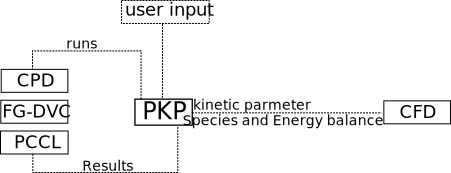
\includegraphics[height=5cm,angle=0]{Fig/scheme}
\caption{scheme of the functioning of \PKP}
\label{F_scheme}
\end{figure}


\begin{figure}[h!]
\centering
\includegraphics[height=7cm,angle=0]{Fig/Fit_result_CO2_Y}
\caption{A plot of the yielded carbon dioxide. The green curve is the fitted single step Arrhenius expression, the blue one the \CPD output. The used feedstock is a Guasare Coal.}
\label{F_FitWaterY}
\end{figure}

%\printbibliography[heading=bibintoc]
\end{document}
